% Type of the document is an article
\documentclass{article}

% use a graphics package for including images
\usepackage{graphicx}

% begin the document
\begin{document}

% give the document a title
\title{IL35620 Website Proposal}

% list the author of the document
\author{Daniel Atkinson}
\date{March 14, 2013}
% print the title, author, etc... here
\maketitle

% start the abstract
%\begin{abstract}
%The abstract of the document should be detailed here
%end the abstract
%\end{abstract}

\tableofcontents
\newpage
Dear Managing Director of Ceredigion Lake Activity Centre
The purpose of this document is to provide information about implementing a website for the activity centre.  This will include benefits of having a websiteand resources required to provide such a service.

\section{Introduction}
Ceredigion Lake Activity Centre is a small organisation with less than 30 employees.  It provides basic activity services such as a swimming pool, tennis courts and a gym.
\\As well as providing these basic services the centre also offers spaces to hire for independant groups to host activities such as fitness classes or self defence classes.  Along with these spaces the centre offers various outdoor activities.
\\The organisational structure consists of a manager overseeing all major operations including public events.  Serveral activity specialists who run the events themselves and aid the public with using equipment and participating in the activities, some medical staff to treat injuries and the rest of the staff oversee al other operations.
\section{What we have}
Currently there is just a noticeboard in the reception area to provide information about upcomming events taking place at the centre, there is also a pile of leaflets providing information about the events hosted at the centre either by the administration itself or by external providers using the centre as a venue.
\\Enquires about events or booking facilities for hosting an event can be made either in person or over the phone.

\section{What we do not have}
We do not have any way to communicate upcoming events to the public who are not on the premisis or who have not called to enquire.
\\Also we do not currently have any means of collecting feedback about the events hosted at the centre.  People can communicate verbally with a mmber of staff about their experiences but unless they also communicate this with other members of the public as well on a mass scale there is very little way of promoting the offered services.  This lack of feedback is very poor.
\\\\Members of the public should be able to see how other people found the services to decide if they would also like to use them.  The feedback would also be usefull to the administration.  The centre could use surveys to collect information about the user experiences and identify what improvements or changes need to me made.

%\section{Why we need web presence}
\section{Advantages}
There are many advantages of having an online presence:
\begin{itemize}

\item Advertising
\\This will allow the centre to more actively advertise upcoming events and put emphasis on the events we want to push more than others

\item Provide Information
\\Enable the centre to provide information about the provided services any time of the day to any person with access to an internet connection.

\item Feedback
\\Allow the public to give the centre feedback on the services it provides
\\This feedback can be seen by other members of the public which can help guide them to the right activity for them or even convince them they want to go to any at all.

\item Contact
\\Allows the public to contact the centre in a more convenient medium than walking into the centre itself or by telephone which both require the time of contact to be while the premisis is open.

\item Hire Services
\\External groups can apply to hire a room or a service via the website.

\end{itemize}
The website will enable much easier communication with the public and provide a feedback channel to help improve the synergy between the organisation and its members.
\\Revenue could also potentialy be increased by providing paid advertising on the website for external groups providing events in our centre.  This would have to be manually approved and not some automated service due to the wide range of people who could be viewing the site and the risk of inapproriate conntent being rather high.  Also the legal connotations linked with certain content that a third party may put in an advertising slot, these must be approved by an experienced member of staff.
\section{Disadvantages}
There are some dissadvantages to an online presence:
\begin{itemize}
\item Staff
\\May need additional staff such as a webmaster to manage the site, current staff may need additional training to add or manage their own content on the website.  Also some existing members of staff may have additional responsibilities due to their content on the site.

\item Cost
\\There are extra costs involved in the business of having a web presence.  There are hosting costs, hiring a web designer or webmaster and/or staff spend time submitting their content when they could be performing their normal duties.
\\This adds either time or monetary costs to the centre in order to maintain a web presence.

\end{itemize}

\section{Website needs}
One of the main requirements of the website is to provide information, this would include:
\begin{itemize}
\item How to apply for membership
\item Cost of membership
\item Cost of events
\item Cost of hiring equipment
\item How to advertise
\item Upcomming events
\item Public Feedback
\item promotions
\end{itemize}

The need to create and maintain a good relationship with the public and keep a clear line of communication open is vital.  A big part of this is to allow users to submit their own content to keep them engaged and to take their opinions onboard to craft our services to suit the needs of our customers.
\\\\A proffessional looking website can be seen as a sign of success and people feel more comfortable using the services of a business that is seen as successfull and professional as it implies quality.  Due to what seems like people having an adiction to social media websites, integration to some of these would be beneficial and increase awareness of our organisation.  This will also make us seem up to date and keeping up with current technologies and not just small time stuck in our ways, that we are open to change.

\section{Target Demographic}
The target demographic for the site will be very wide spread.  It will be aimed at children for after school activities, to teenagers for general fitness and recreational activities, or just for anybody who wishes to keep up their general fitness.  It is also open to anybody who wants to participate in any of the external activities hosted such as self defence classes.  All of these such events have a wide age range from very young to the elderly and include members of both genders.
\\From a financial standpoint the centre focuses on a low to medium range of income by providing affordable services and also providing for more costly activities.
\\This displays a large cross-over where some services are for all age ranges but others are focuses to smaller groups but overall ther is a very large age range and wide target and as such all content must be suitable for all of these cases.

\section{Technical}
Reccomendations I would like to make regarding to the features the website should have:
\begin{itemize}
\item Search
\\The header of all pages should contain a search bar to allow the users to more easily find content throughout the site.

\item Map
\\A map to show the centres geographical location

\item Integration of social media
\\This could be a twitter feed showing the latest posts made on the centres twitter feed.

\item Tag cloud
\\To allow the users to see what the most popular terms other users have been searching for.

\item Survey
\\Allowing to users of the site to provide us with feedback on their experiences of our services.

\item Analytics
\\The use of a web analytics tools such as Google analytics could be used to gather information such as how many people have visited the site and which pages are the most popular.

\item Navigation
\\Breadcrumbs will be used so that the user knows where they are in the site at all times as to not get lost.  A sitemap will also be used to aid in navigation fo the site.  A smooth navigation of the site will help keep users and help make sure they do not get frustrated and leave due to not being able to do what they want.
\\The broad and shallow approach will be taken due to the results of creating an IA diagram (Found in Appendix A).  There is a moderate amount of content but most of which is not related to each other and would need its own section at the same level of navigation.

\item Accessibillity
\\This will ensure that users with disabilities will still eb able to use the site due to text resizing for the visually impaired users and alt tags on images also contrast settings.  These also adress some legal issues that could arise if we do not address these.  Certain equality groups have taken legal action against website hosts in the past for not implementing such accessibility features.

\item Archives
\\Webnode is the proposed host for this project and as such the responisbility of maintaining the archives of the site falls to them.

\end{itemize}
\section{Legal}
Due tot he fact that the centre is the author of the content on the website there should be no copyright issues but the content submitted by the external groups advertising on the site will need to reference their content according to the proper licence such as creative commons whcih is the most commonly reference on sites of this type.
\\Any information held by us about our users will be will be handled in accordance to the Data Protection Act.  Due to the fact that we already hold information on our members the Data Protection Act should be nothing new to our staff.
\\\\Features of the site such as users being able to post information about their experiences of the services we provide, the centre can be held accountable for what users may post on the site, for this reason a terms and conditions page must be in place to help ensure that users know that all content they submit it their own reponsibility and not that fo the centre.  It is of course our responsibility to remove any offensive or legaly infringing content once made aware of it.

\section{Resources}
Some members of staff will need to be given additional responsibilities to manage content on the site relevant to the activities they run.  They will also need to respond to relevant queries recieved via the website and the centre twitter account.  Due to giving each member of staff their own responsibilities on the site we will not have to hire a permanent webmaster after the inital build of the site as this could be very costly and would be un-neccesary as long as our staff have an acceptable level of technical knowledge to enable them to maintain their relevant content.
\\Once the website ahs been completed training should be carried out with every staff member who will be providing input into the sites content.
\\\\An individual member of staff will filter the content being published to the site to try and ensure that it is all beneficial to the organisation, that it is up to dat eand that it has no negative legal inplications.
\\Regular meetings should be held to discuss and implement changes based on user feedback and these meetings frequency will be determined by the rate and volume of feedback recieved.
\\\\The only charges that should be incured by this project will be the webmaster to initialy create the site, and by Webnode who charge for premium accounts, although the free version content should be adequate for our needs.

\section{Summary}
The maintaining of a website will increase the organisations image and public awareness of the services we offer and the benefits far outweigh the costs involved in implementing this project.  Relations between the organisationand the public will be greatly improved and help give us the image of a modern business who is up to date with current technologies and methods.
\newpage
\section{Apendix A}
\subsection{IA Diagram}
This diagram shows that most of the sites content should not go many layers deep as there are many sections but each one has very limited content.
\begin{figure}[h]
\centering
        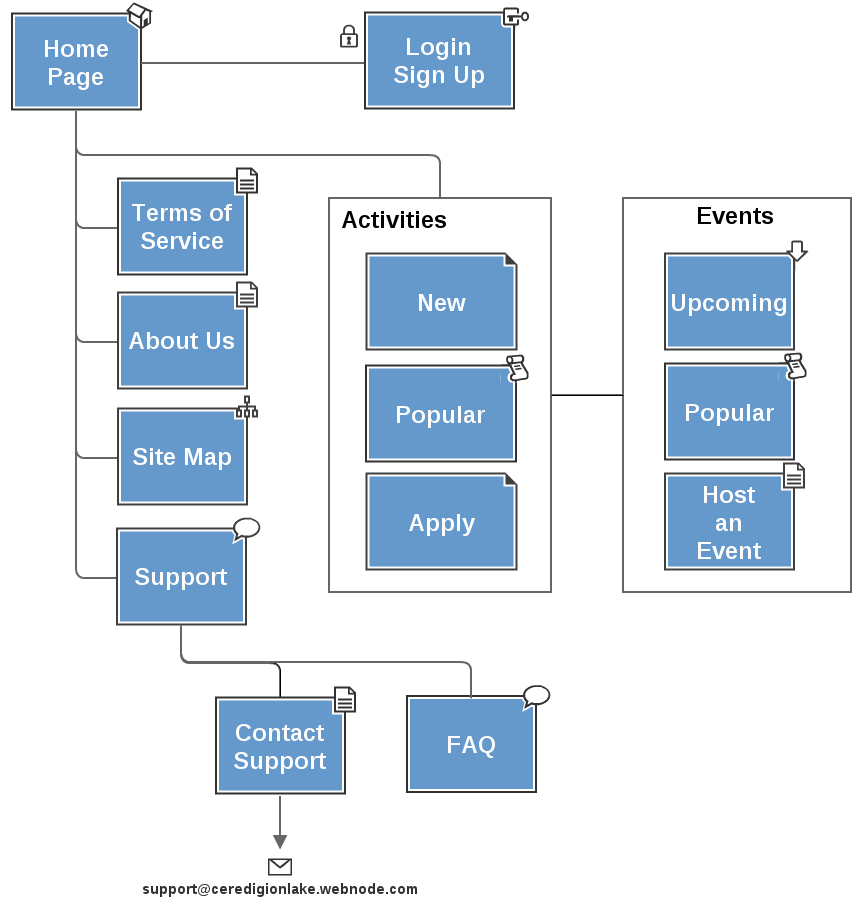
\includegraphics[width=5.0in] {IA.png}
        \caption{IA Diagram}
        \label{IA Diagram}
\end{figure}

% end the document
\end{document}
